\documentclass[times, utf8, zavrsni]{fer}
\usepackage{booktabs}
\usepackage{float}

\begin{document}

% TODO: Navedite broj rada.
\thesisnumber{000}

% TODO: Navedite naslov rada.
\title{Web-aplikacija za rješavanje programskih zadataka s elementima društvene mreže}

% TODO: Navedite vaše ime i prezime.
\author{Nikola Kešćec}

\maketitle

% Ispis stranice s napomenom o umetanju izvornika rada. Uklonite naredbu \izvornik ako želite izbaciti tu stranicu.
\izvornik

% Dodavanje zahvale ili prazne stranice. Ako ne želite dodati zahvalu, naredbu ostavite radi prazne stranice.
\zahvala{Srdačno se zahvaljujem svojem mentoru, prof. dr. sc Igoru Mekteroviću na cijenjenoj pomoći, savjetovanju i stručnom usmjeravanju. Također se zahvaljujem i Hermanu-Zvonimiru Došiloviću na pomoći i uputama oko Judge0-a bez kojeg ovaj završni rad ne bi bio moguć.}

\tableofcontents

\chapter{Uvod}
Sveprisutnost računalnih sustava tijekom početka drugog tisućljeća uveliko je doprinijela većem porastu zanimacije populacije prema svemu što je povezano s računalima.  Naravno, to podrazumijeva i čin \textbf{programiranja}. Programiranje možemo opisati kao čin dizajniranja i razvoja izvršnog računalnog programa čija je svrha uspješno postizanje specifičnog računskog rezultata ili odrada specifičnog zadatka.\\
Iako su već početkom tisućljeća računalni sustavi bili poprilično sveprisutni, neusporedivo je koliko je njihova zastupljenost u svakodnevnom ljudskom životu porasla. Porastom njihove zastupljenosti porasla je potražnja za računalnom sklopovskom podrškom \engl{hardware}, a s njom i potreba za kvalitetnom programskom podrškom \engl{software}. Kvalitetna programska podrška rezultat je godina učenja, razmatranja i pisanja programskog koda, a kao i svaku drugu vještinu potrebno ju je održavati. Održavanje je moguće na mnogo načina, a podosta popularan način usavršavanja i održavanja vještosti pisanja programskog koda jest rješavanje programskih zadataka. Naravno, sva rješenja programskih zadataka nisu jednako kvalitetna stoga se nerijetko rješenja rangiraju po kvaliteti sa svrhom isticanja znanja autora kvalitetnog rješenja. Natjecateljski ljudski duh proizveo je događanja na kojima se upravo takav pristup prakticira i cijeni, znana još kao i programerska natjecanja \engl{competitive programming competitions}.\\
Makar su takva događanja izrazito bogat izvor programerskog znanja, programiranjem zainteresirana neiskusna populacija teško da će svojevoljno ući na opisana događanja. Razlog tome je razlika u količini znanja između njih i regularnih sudionika jer dobar dio tih sudionika već je vrlo vješt. Stoga je postojanje internetskih stranica koje pružaju uvid u programiranje i rješavanje programskih zadataka dobrodošla novost. Ipak, često riječ vrlo iskusnog programera neiskusnom programeru može biti neprocjenjiva. Iz tog razloga zanimljiv je spoj socijalnih mreža \engl{social networks} i stranica koje pružaju mogućnost rješavanja programskih zadataka. Osobi koju pisanje programskog koda interesira stranica pruža nekompetitivnu mogućnost rješavanja zadataka, a iskusnom programeru mogućnost da kroz rješavanje i objašnjavanje svojih rješenja produbi i utemelji svoja znanja. Upravo je takva kombinacija osnovnih elemenata  spomenutih stranica tema ovog završnog rada te joj je ime \textbf{Codeflow}.

\chapter{Korisnički zahtjevi}
Internetska stranica koja kombinira elemente socijalnih mreža i elemente stranica s tematikom programskog koda treba omogućiti korisniku ispunjavanje mješavine elementarnih \textbf{funkcionalnih} i \textbf{nefunkcionalnih} zahtjeva koje stranice oba navedena tipa ispunjavaju. 
	\section{Funkcionalni zahtjevi}
	Funkcionalni zahtjevi podrazumijevaju usluge koje sustav mora pružati te kako će reagirati na različite ulazne poticaje. Drugim riječima, funkcionalni zahtjevi definiraju što internetska stranica može učiniti za određenog korisnika i što određeni korisnici mogu učiniti na njoj.
	Većina modernih socijalnih mreža traže od svojih korisnika da prvo naprave korisnički račun prije nego što im dopuste pristup njihovim glavnim funkcionalnostima. Analogno tako treba tražiti i Codeflow, stoga na korisnika treba gledati na dva načina; kao na \textbf{neregistriranog korisnika} i \textbf{registriranog korisnika}.
	
		\subsection{Zahtjevi neregistriranog korisnika}
		Neregistriran korisnik, prema uzoru na mnoge moderne socijalne mreže, ima mogućnost pristupanja stranici dobrodošlice te pravo registriranja. Neregistrirani korisnik tijekom registracije treba upisati određene podatke s kojima će se, ako su ispravni te nakon što se njegov korisnički račun napravi, prijaviti. Činom registracije neregistrirani korisnik postaje registriran. Grafički prikaz zahtjeva prikazan je na slici \ref{fig:zahtjevi-nereg}.
		
		\begin{figure}[H]
			\centering
			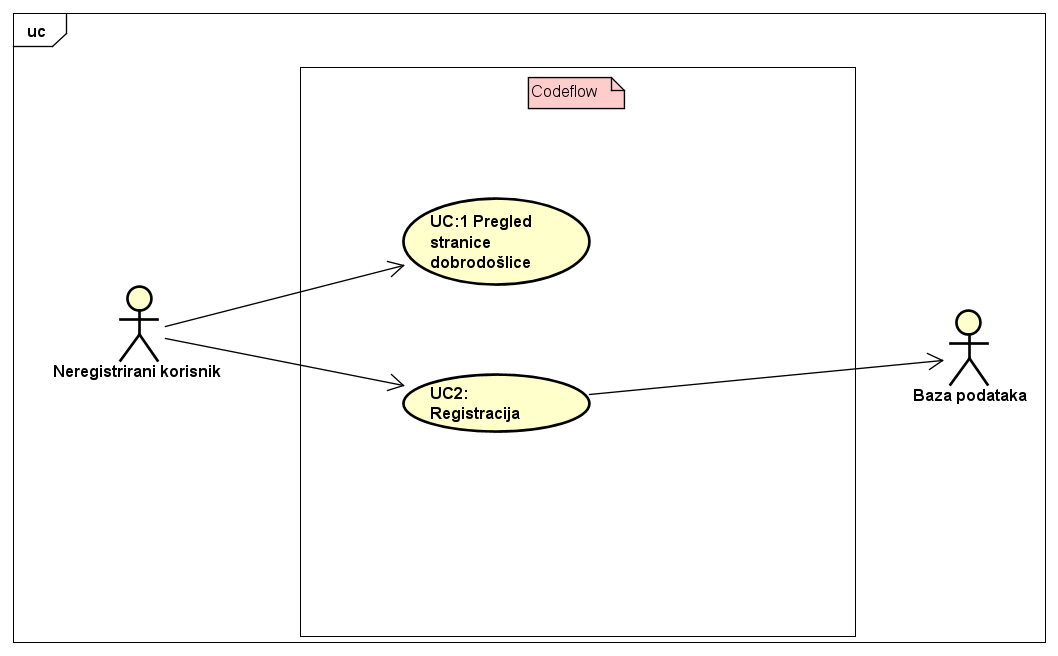
\includegraphics[width=\linewidth]{pictures/zahtjevi/nereg_korisnik.png}
			\caption{Zahtjevi neregistriranog korisnika}
			\label{fig:zahtjevi-nereg}
		\end{figure}
		
		\subsection{Zahtjevi registriranog korisnika}
		Nakon što se korisnik registrira broj zahtjeva koje Codeflow korisniku treba ispuniti raste. Registriranom korisniku mogućnost prijave s podacima koje je koristio za registraciju mora biti dostupna te nakon što se prijavi opcija pregledavanja ponuđenih zadataka i rang liste treba biti podržana. Ponuđene zadatke treba moći filtrirati na neki od dostupnih načina i Codeflow registriranom korisniku treba nuditi mogućnost detaljnijeg pregleda jednog od filtriranih zadataka. Codeflow treba prema uzoru na moderne socijalne mreže nuditi filtriranje prema sljedećim kriterijima: 
		\begin{itemize}
			\item preporučeni zadaci
			\item zadaci slijeđenih korisnika
			\item najnoviji zadaci
		\end{itemize}
		Tijekom detaljnijeg pregleda odabranog zadatka registriranom korisniku moraju biti ponuđene opcije ocjenjivanja i komentiranja zadatka. Uz sam detaljniji opis zadatka, korisniku treba biti omogućen odabir nekog od rješenja gledanog zadatka. Odabrano rješenje registrirani korisnik također mora biti u mogućnosti komentirati, a mogućnost ocjenjivanja zadatka treba mu biti omogućena samo nakon rješavanja zadatka. Budući da je rješavanje zadatka preduvjet jednom od ostalih zahtjeva, ta funkcionalnost  korisniku svakako treba biti omogućena. Korisničko rješenje aplikacija mora evaluirati pomoću vanjskog izvršitelja programskog koda te nakon evaluacije spremiti. Uz stvaranje rješenja programskih zadataka, aplikacija registriranom korisniku treba ponuditi i opciju stvaranja programskog zadatka. Zahtjevi navedeni uz pregledavanja zadataka, rješavanje zadataka i stvaranje zadataka jezgreni su zahtjevi koje Codeflow mora obavezno podržavati.\\ Registriranom korisniku mogućnost potpunog upravljanja vlastitim zadacima, rješenjima, komentarima i ocjenama mora biti dostupna. Pod tim se podrazumijevaju  mogućnosti njihovog uređivanje i brisanja. Uz navedenu mogućnost upravljanja vlastitim zadacima, rješenjima, komentarima i ocjenama, registriranom korisniku mora biti omogućeno mijenjanje vlastitih podataka. Po uzoru na određene mogućnosti modernih socijalnih mreža, registriranom korisniku opcija pregleda profila drugih registriranih korisnika treba biti dostupna, a moguće praćenje ili otpraćivanje željenih korisnika također treba biti podržano. Osim mogućnosti pregleda tuđih korisničkih stranica, registrirani korisnik isto tako treba moći vidjeti svoju korisničku stranicu. Detaljniji grafički prikazi ovih korisničkih zahtjeva vidljivi su na slikama \ref{fig:zahtjevi-korisnik1} i \ref{fig:zahtjevi-korisnik2}.
		
		\begin{figure}[H]
			\centering
			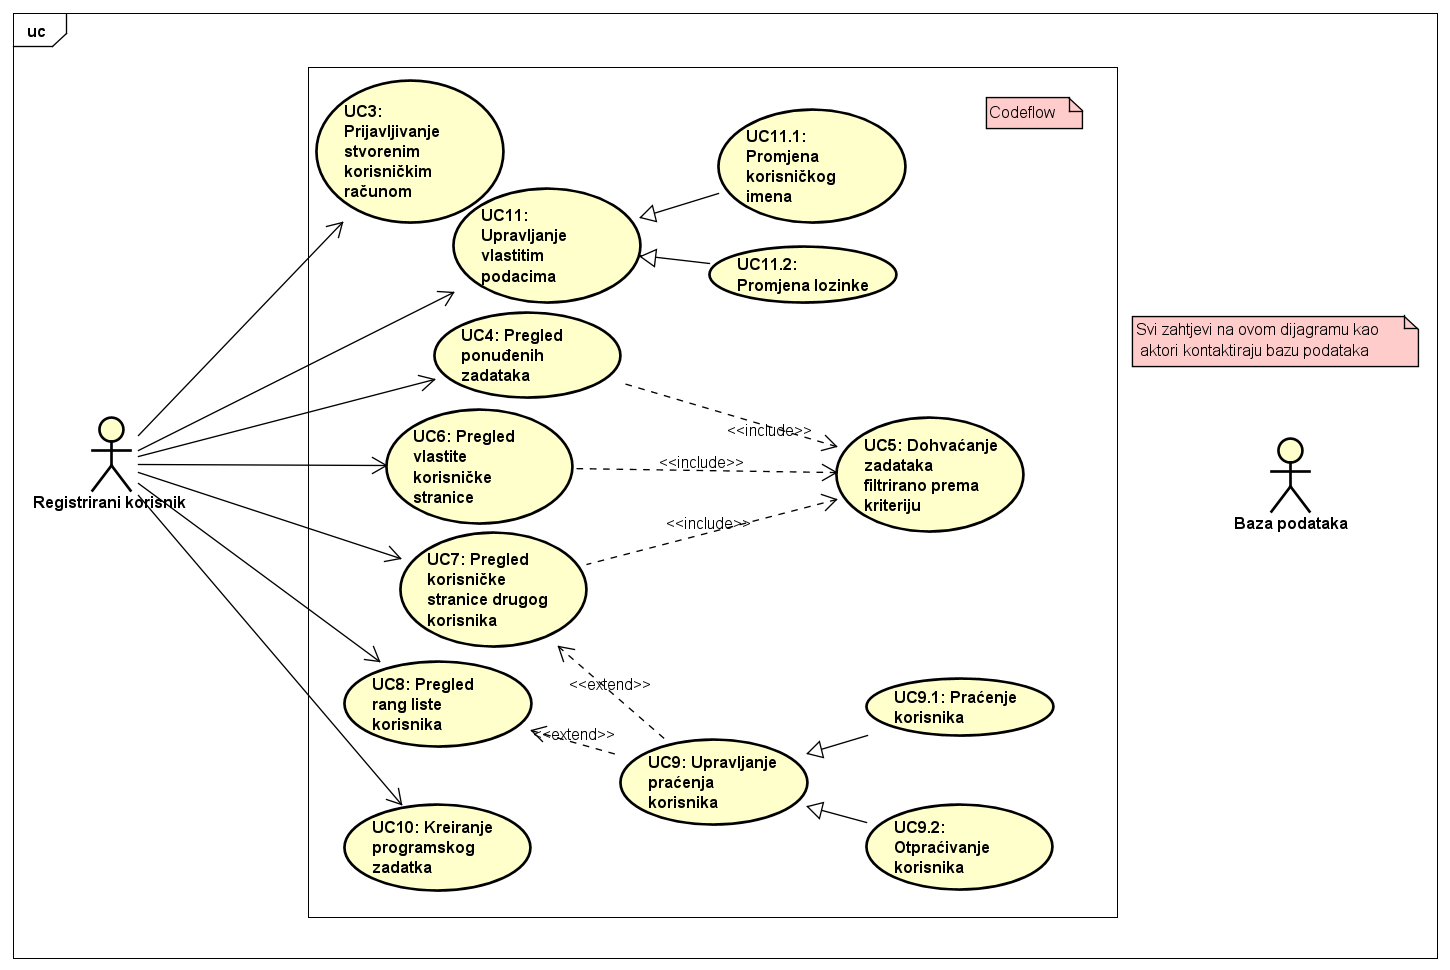
\includegraphics[width=\linewidth]{pictures/zahtjevi/korisnik1.png}
			\caption{Zahtjevi registriranog korisnika, prvi dio.}
			\label{fig:zahtjevi-korisnik1}
		\end{figure}
		
		\begin{figure}[H]
			\centering
			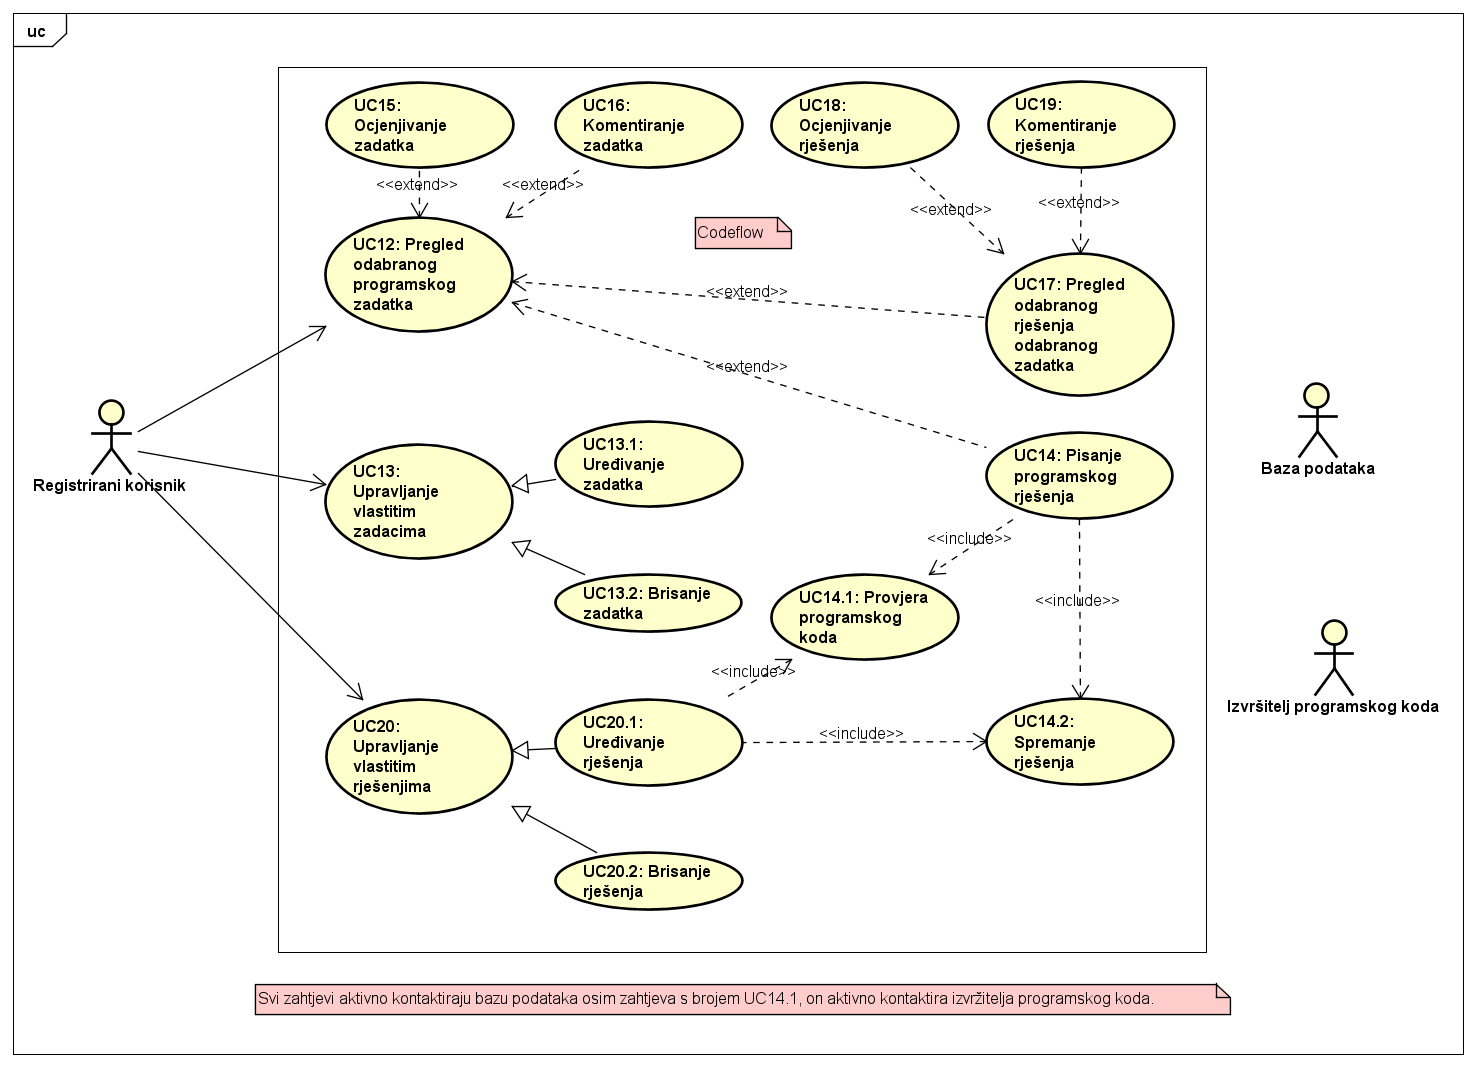
\includegraphics[width=\linewidth]{pictures/zahtjevi/korisnik2.png}
			\caption{Zahtjevi registriranog korisnika, drugi dio.}
			\label{fig:zahtjevi-korisnik2}
		\end{figure}
	
	\section{Nefunkcionalni zahtjevi}
	Nefunkcionalni zahtjevi, za razliku od funkcionalnih, ne opisuju koje mogućnosti sustav treba pružati nego koje karakteristike on treba imati. U slučaju tipa promatrane internetske stranice, nefunkcionalni zahtjevi navedeni su unutar sljedeće liste:
	\begin{itemize}
		\item korisničke lozinke trebaju biti pravilno spremljene
		\item veza s bazom podataka i izvršiteljem programskog koda treba biti stabilna
		\item korisničko sučelje treba biti intuitivno za korištenje
		\item ostvarivanje evaluacije korisničkih rješenja treba biti unutar dvominutnog intervala 
	\end{itemize}
\chapter{Postojeća programska rješenja te uvođenje socijalnih elemenata}
Već postojeća programska rješenja iz kojih Codeflow uvelike pronalazi inspiraciju za funkcionalnostima su sljedeća:
\begin{itemize}
	\item Leetcode
	\item Edgar
	\item Codewars
	\item HackerRank
\end{itemize}
U nastavku svako od navedenih programskih rješenja bit će pobliže razmotreno.
	\section{Leetcode}
	Leetcode vjerojatno je najveća i najpoznatija internetska stranica koja omogućava rješavanje programskih zadataka. Osnovana 2015. godine u Silicijskoj dolini, od samog početka bilježila je značajan rast i već 2017. godine imala preko milijun registriranih korisnika.\\
	Svrha i namjera Leetcode stranice jest priprema korisnika stranice na razgovore za posao pomoću specifično dizajniranih programskih zadataka. Pripremljeni zadaci slične su prirode kao i oni koje najpoznatije tehnološke firme predstavljaju svojim pristupnicima na razgovorima za posao. Preduvjet pristupu ponuđenim zadacima je registracija, a registrirani korisnici uz mogućnost rješavanja zadataka (koje također mogu filtrirati po kriterijima) također mogu provoditi diskusije unutar foruma. Diskusije su često povezane s temom pitanja koje velike tehnološke tvrtke postavljaju. Bitno je napomenuti da Leetcode podržava programska rješenja pisana unutar četrnaest različitih programskih jezika. Rješenja zadataka također mogu biti predložena unutar diskusijskog foruma te dodatno komentirana od drugih korisnika.\\
	Uz sve navedene funkcionalnosti koje Leetcode nudi, također neke funkcionalnosti izostavlja. Leetcode ne dopušta svojim registriranim korisnicima da sami dizajniraju svoje zadatke ili da prate korisnike koji su im se veoma dojmili unutar diskusijskog foruma.\\
	Ukratko, Leetcode internetska stranica veoma je impresivna po broju funkcionalnosti koje nudi svojim registriranim korisnicima. Navedene funkcionalnosti napisane unutar ove sekcije najosnovnije su mogućnosti koje Leetcode nudi.
	\begin{figure}[H]
		\centering
		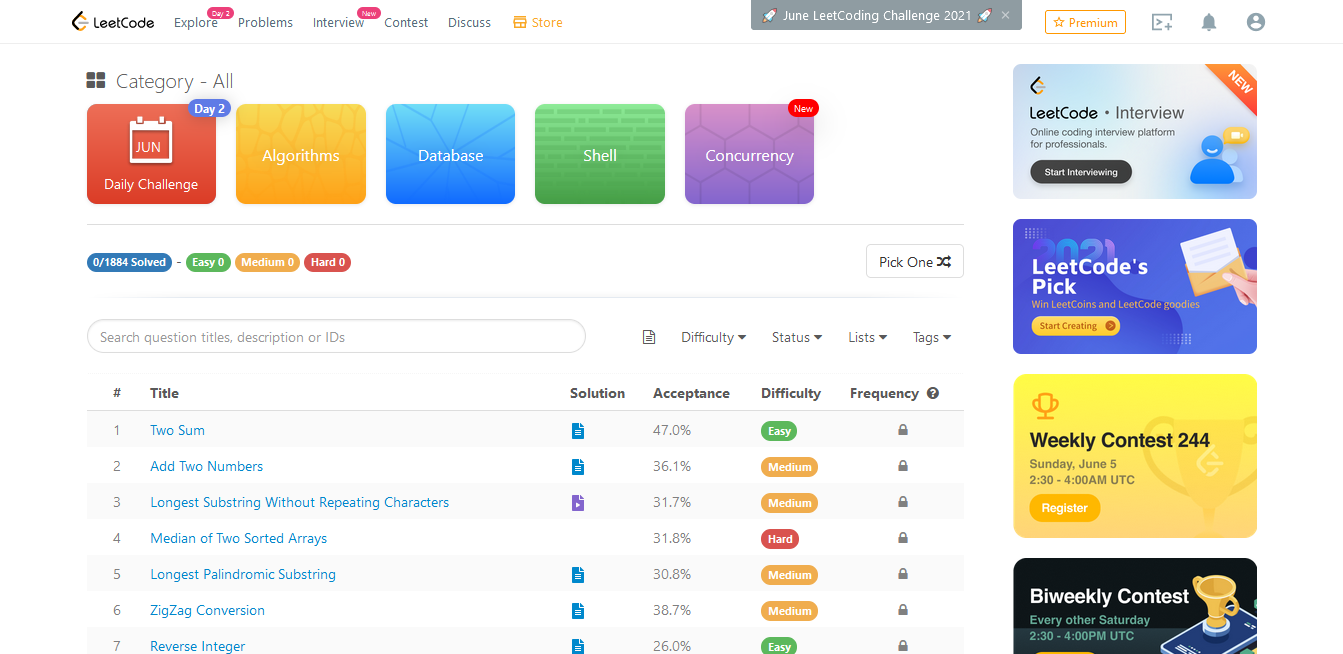
\includegraphics[width=\linewidth]{pictures/prikazi/Leetcode.png}
		\caption{Prikaz stranice Leetcode}
		\label{fig:leetcode}
	\end{figure}

	\section{Edgar}
	Edgar je internetska stranica koju Fakultet Elektrotehnike i Računarstva koristi u edukacijske svrhe, primarno kao sustav provođenja provjera vezanih uz temu programiranja. Razvijen na Fakultet Elektrotehnike i Računarstva, u velikoj je uporabi zbog svoje mogućnosti definiranja i provođenja testova. \\
	Pristup internetskoj stranici moguć je samo ovlaštenim osobama pomoću njihovih korisničkih računa. Korisnici koji imaju ulogu predavača mogu definirati testove koje onda ostali korisnici (koji nisu predavači) rješavaju. Edgar podržava mnoge programske jezike te tijekom rješavanja testnih zadataka vraća povratne informacije korisniku. Također, Edgar podržava stvaranja edukacijskih materijala poput edukacijskih vježbi. Isto tako, korisniku je na raspolaganju i pisanje proizvoljnog koda unutar "Code sandbox" funkcionalnosti stranice. Korisnici Edgara ne mogu ući u interakciju jedni s drugima.\\
	Internetska stranica Edgar primarno pruža funckionalnosti provjere programskog koda. Ne fokusira se na interakciju korisnika te sadržava poveći broj funkcionalnosti od kojih je ovdje nekoliko navedeno.
	\begin{figure}[H]
		\centering
		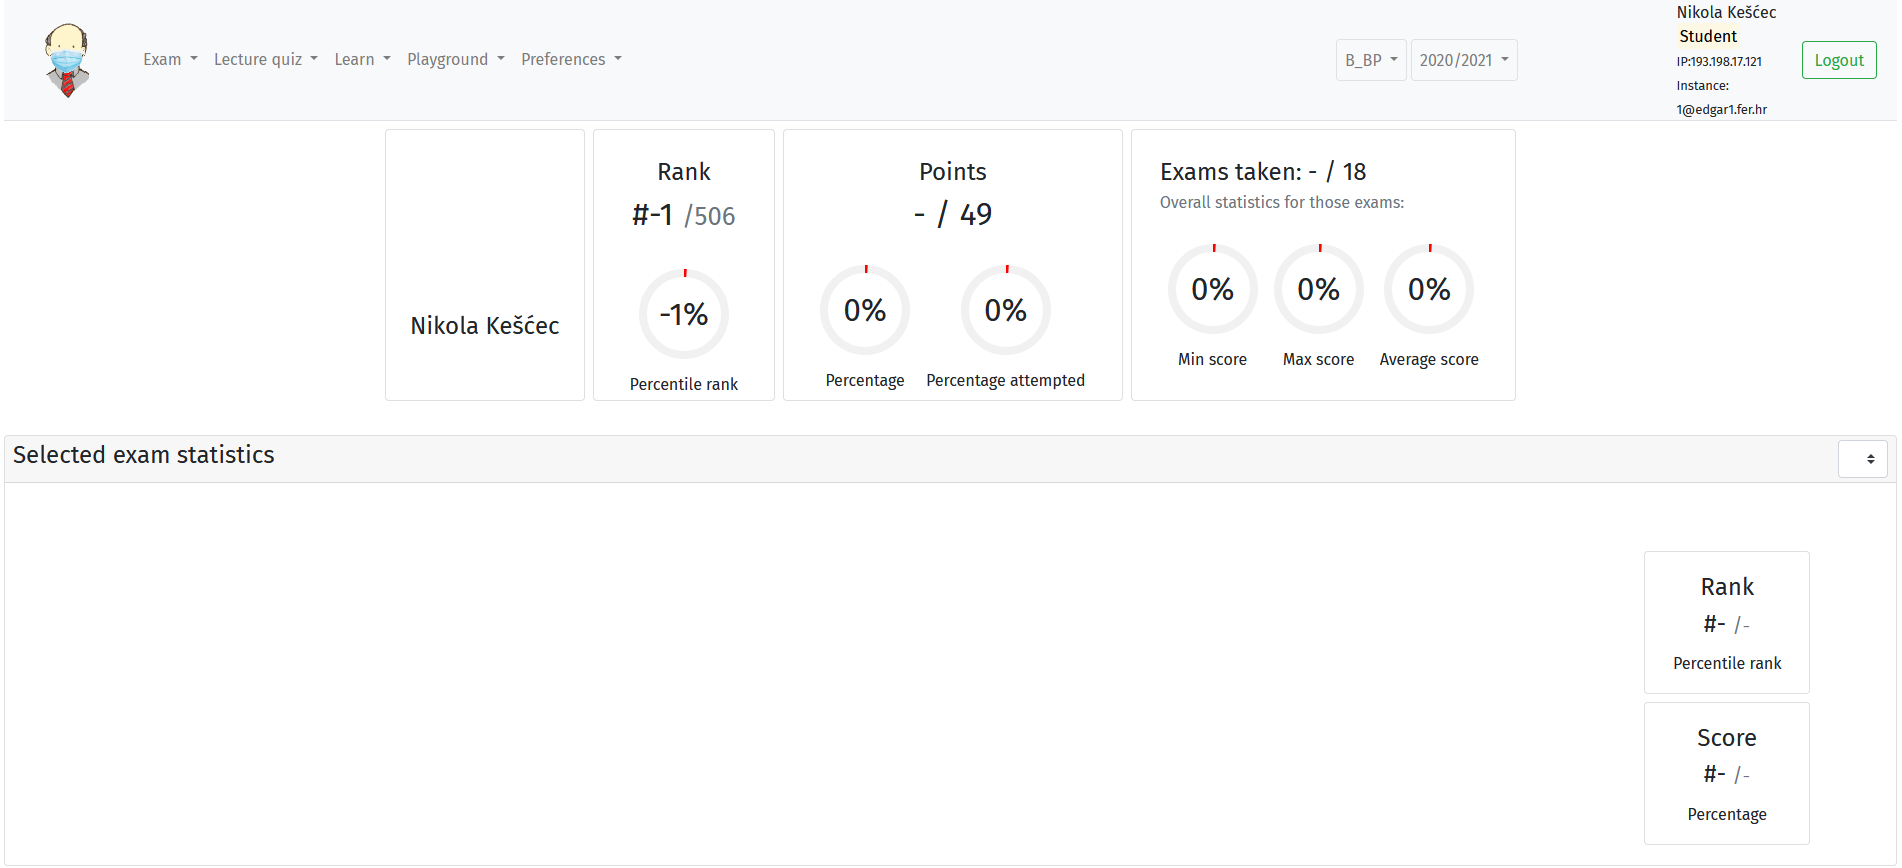
\includegraphics[width=\linewidth]{pictures/prikazi/Edgar.png}
		\caption{Prikaz stranice Edgar}
		\label{fig:edgar}
	\end{figure}
	
	\section{Codewars}
	Codewars internetska stranica po funkcionalnosti slična je Leetcodeu, ali uvodi dodatne mogućnosti rangiranja korisnika prema težini zadataka koje rješavaju (zvani \textit{kata}). Osnovana je 2012. godine, a  njezina namjera usavršavanje je znanja programskih jezika i proširenje znanja drugih jezika.\\
	Kate su zadaci koji nose određenu količinu bodova, a definiraju ih korisnici Codewarsa. Svaka kata nosi odrežen broj bodova, zvani \textit{kyu}. Teži zadaci nose više bodova, a rješenja zadataka moguće je komentirati s ostalim korisnicima. Također, isto kao i sve već spomenute internetske stranice, Codewars pružaju mogućnost rješavanja zadataka u različitim jezicima. Bitno je napomenuti da Codewars implementira sve popularniji proces "igrifikacije" \engl{gamification}. Taj proces uvodi razine i određene nagrade koje korisnike motiviraju za daljnje rješavanje sve težih zadataka.\\
	Tijekom registracije, korisnici trebaju proći inicijalizacijski test koji testira njihova osnovna znanja jednog od ponuđenih jezika i to je minimalno predznanje glavan je preduvjet budućeg korištenja stranice.
	
	\section{HackerRank}
	Internetska stranica HackerRank pruža drugačije usluge od već navedenih stranica. Namjera stranice je povezivanje programera s tvrtkama koje bi bile zainteresirane za njih, ali i učenje novih jezika, programskih algoritama te paradigmi.\\
	Stranica pruža mogućnost stvaranja računa korisnicima, ali i tvrtkama koje interesira HackerRank. Mogućnost rješavanja programskih zadataka omogućena je za korisnike i tvrtke, a nerijetko stranica organizira i natjecanja zvana "CodeSprints". Na tim natjecanjima korisnici rješavaju iste programske zadatke. HackerRank stranica predana rješenja rangira prema njihovoj točnosti i kvaliteti. Autore tih rješenja također rangira na HackerRank ljestvici korisnika, te, kao i Codewars, provodi proces "igrifikacije".\\
	Mogućnosti HackerRank stranice raspodijeljene su između različitog tipa korisnika: regularnog korisnika i tvrtke. Korisnicima pruža mogućnosti rješavanja zadataka u svrhu promocije te onim korisnicima koji traže posao potencijalno može pomoći u tomu.
	\begin{figure}[H]
		\centering
		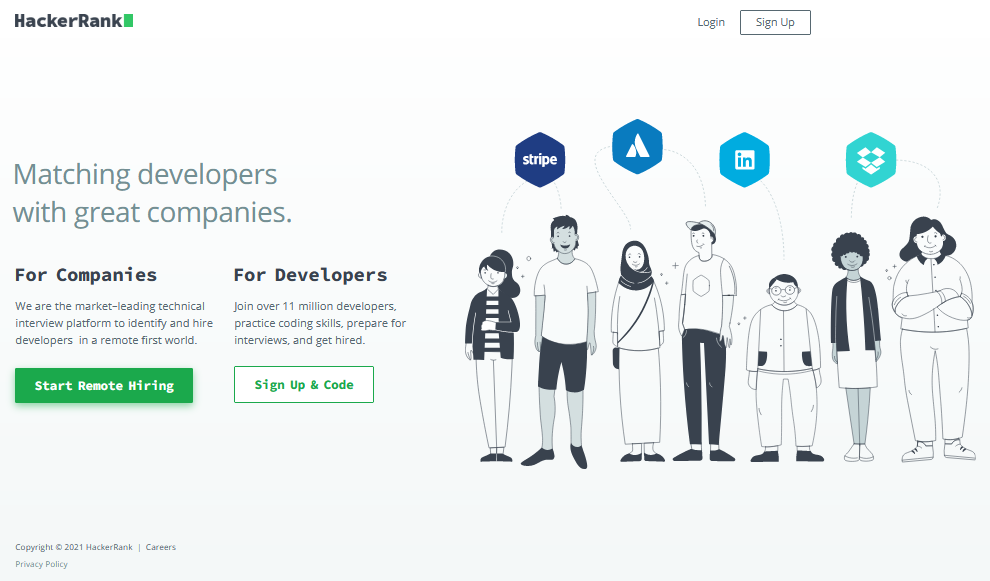
\includegraphics[width=\linewidth]{pictures/prikazi/HackerRank.png}
		\caption{Prikaz stranice dobrodošlice HackerRank internetske stranice}
		\label{fig:hackerrank}
	\end{figure}
	
	\section{Zajedničke funkcionalnosti}
	Vidljivo je iz bližeg razmatranja navedenih stranica da svaka od stranica ima različitu namjeru te u različite svrhe koristi funkcionalnost zadavanja i rješavanja zadataka. Stranice Codewars, Leetcode i HackerRank donekle su slične po funkcionalnostima koje pružaju, ali ipak razlikuju se podosta u namjeri. Edgar je najrazličitiji od navedenih stranica jer njegova je svrha prvenstveno akademske i edukacijske prirode. Ipak, navedene stranice imaju nekoliko najčešćih dijeljenih funkcionalnosti:
	\begin{itemize}
		\item stvaranje zadataka
		\item rješavanje zadataka
		\item provjera zadataka
		\item komentiranje rješenja (Codewars, Leetcode, HackerRank)
	\end{itemize}
	Bitno je također uvidjeti da dio stranica pruža određene mogućnosti socijalnih mreža, kao što su već spomenuto komentiranje rješenja te mogućnost određene interakcije s korisnicima. Ipak, mogućnosti praćenja korisnika kod velikog dijela stranica nisu moguće, a isto tako direktno ocjenjivanje rješenja nije podržano na svim stranicama. Nerijetko su i određene funkcionalnosti stranica moguće samo korisnicima koji plaćaju određenu pretplatu (poput pregleda službenog rješenja nekog programskog zadatka).
	Ono što Codeflow stranica sadržava unutar sebe jest spoj navedenih najčešćih funkcionalnosti promotrenih stranica i jezgrenih funkcionalnosti modernih socijalnih mreža. Te jezgrene funkcionalnosti su:
	\begin{itemize}
		\item praćenje korisnika
		\item komentiranje na objavljene sadržaje drugih korisnika (uključujući vlastite)
		\item ocjenjivanje sadržaja drugih korisnika
		\item pregledavanje profila drugih korisnika
	\end{itemize}


\chapter{Korištene tehnologije}
Moderne internetske tehnologije prilagođene su razvoju sustava koji se pridržava troslojne arhitekture sustava. Moderna troslojna arhitektura sustava sastoji se od:
\begin{itemize}
	\item korisničkog ili prezentacijskog sloja
	\item poslovnog sloja
	\item podatkovnog sloja
\end{itemize}

	\section{Tehnologije prezentacijskog sloja}
	
	\section{Tehnologije poslovnog sloja}

	\section{Tehnologije podatkovnog sloja}
	
	\section{Pomoćne tehnologije}


\chapter{Arhitektura rješenja}
Već postojeća rješenja, njihove značajke te uvođenje socijalnih elemenata

\chapter{Prikaz rješenja}
Već postojeća rješenja, njihove značajke te uvođenje socijalnih elemenata

\chapter{Budući razvitak}
Već postojeća rješenja, njihove značajke te uvođenje socijalnih elemenata

\chapter{Zaključak}
Zaključak.

\bibliography{literatura}
\bibliographystyle{fer}

\begin{sazetak}
Sažetak na hrvatskom jeziku.

\kljucnerijeci{Ključne riječi, odvojene zarezima.}
\end{sazetak}

% TODO: Navedite naslov na engleskom jeziku.
\engtitle{Title}
\begin{abstract}
Abstract.

\keywords{Keywords.}
\end{abstract}

\end{document}
